% !TeX root = ..\..\rapport_13_2.tex
\section{Konklusion} \label{chap:conclusion}
I første version af rapport 1, lagde vi ud med et design af programmet som vist herunder i figur \ref{fig:class_report1}. Her var en \texttt{AppController} ansvarlig for stort set alt, vi ikke kunne pakke ind i de øvrige modeller.
\begin{figure}[H]
    \centering
    \caption{Klassediagram fra rapport 1}
    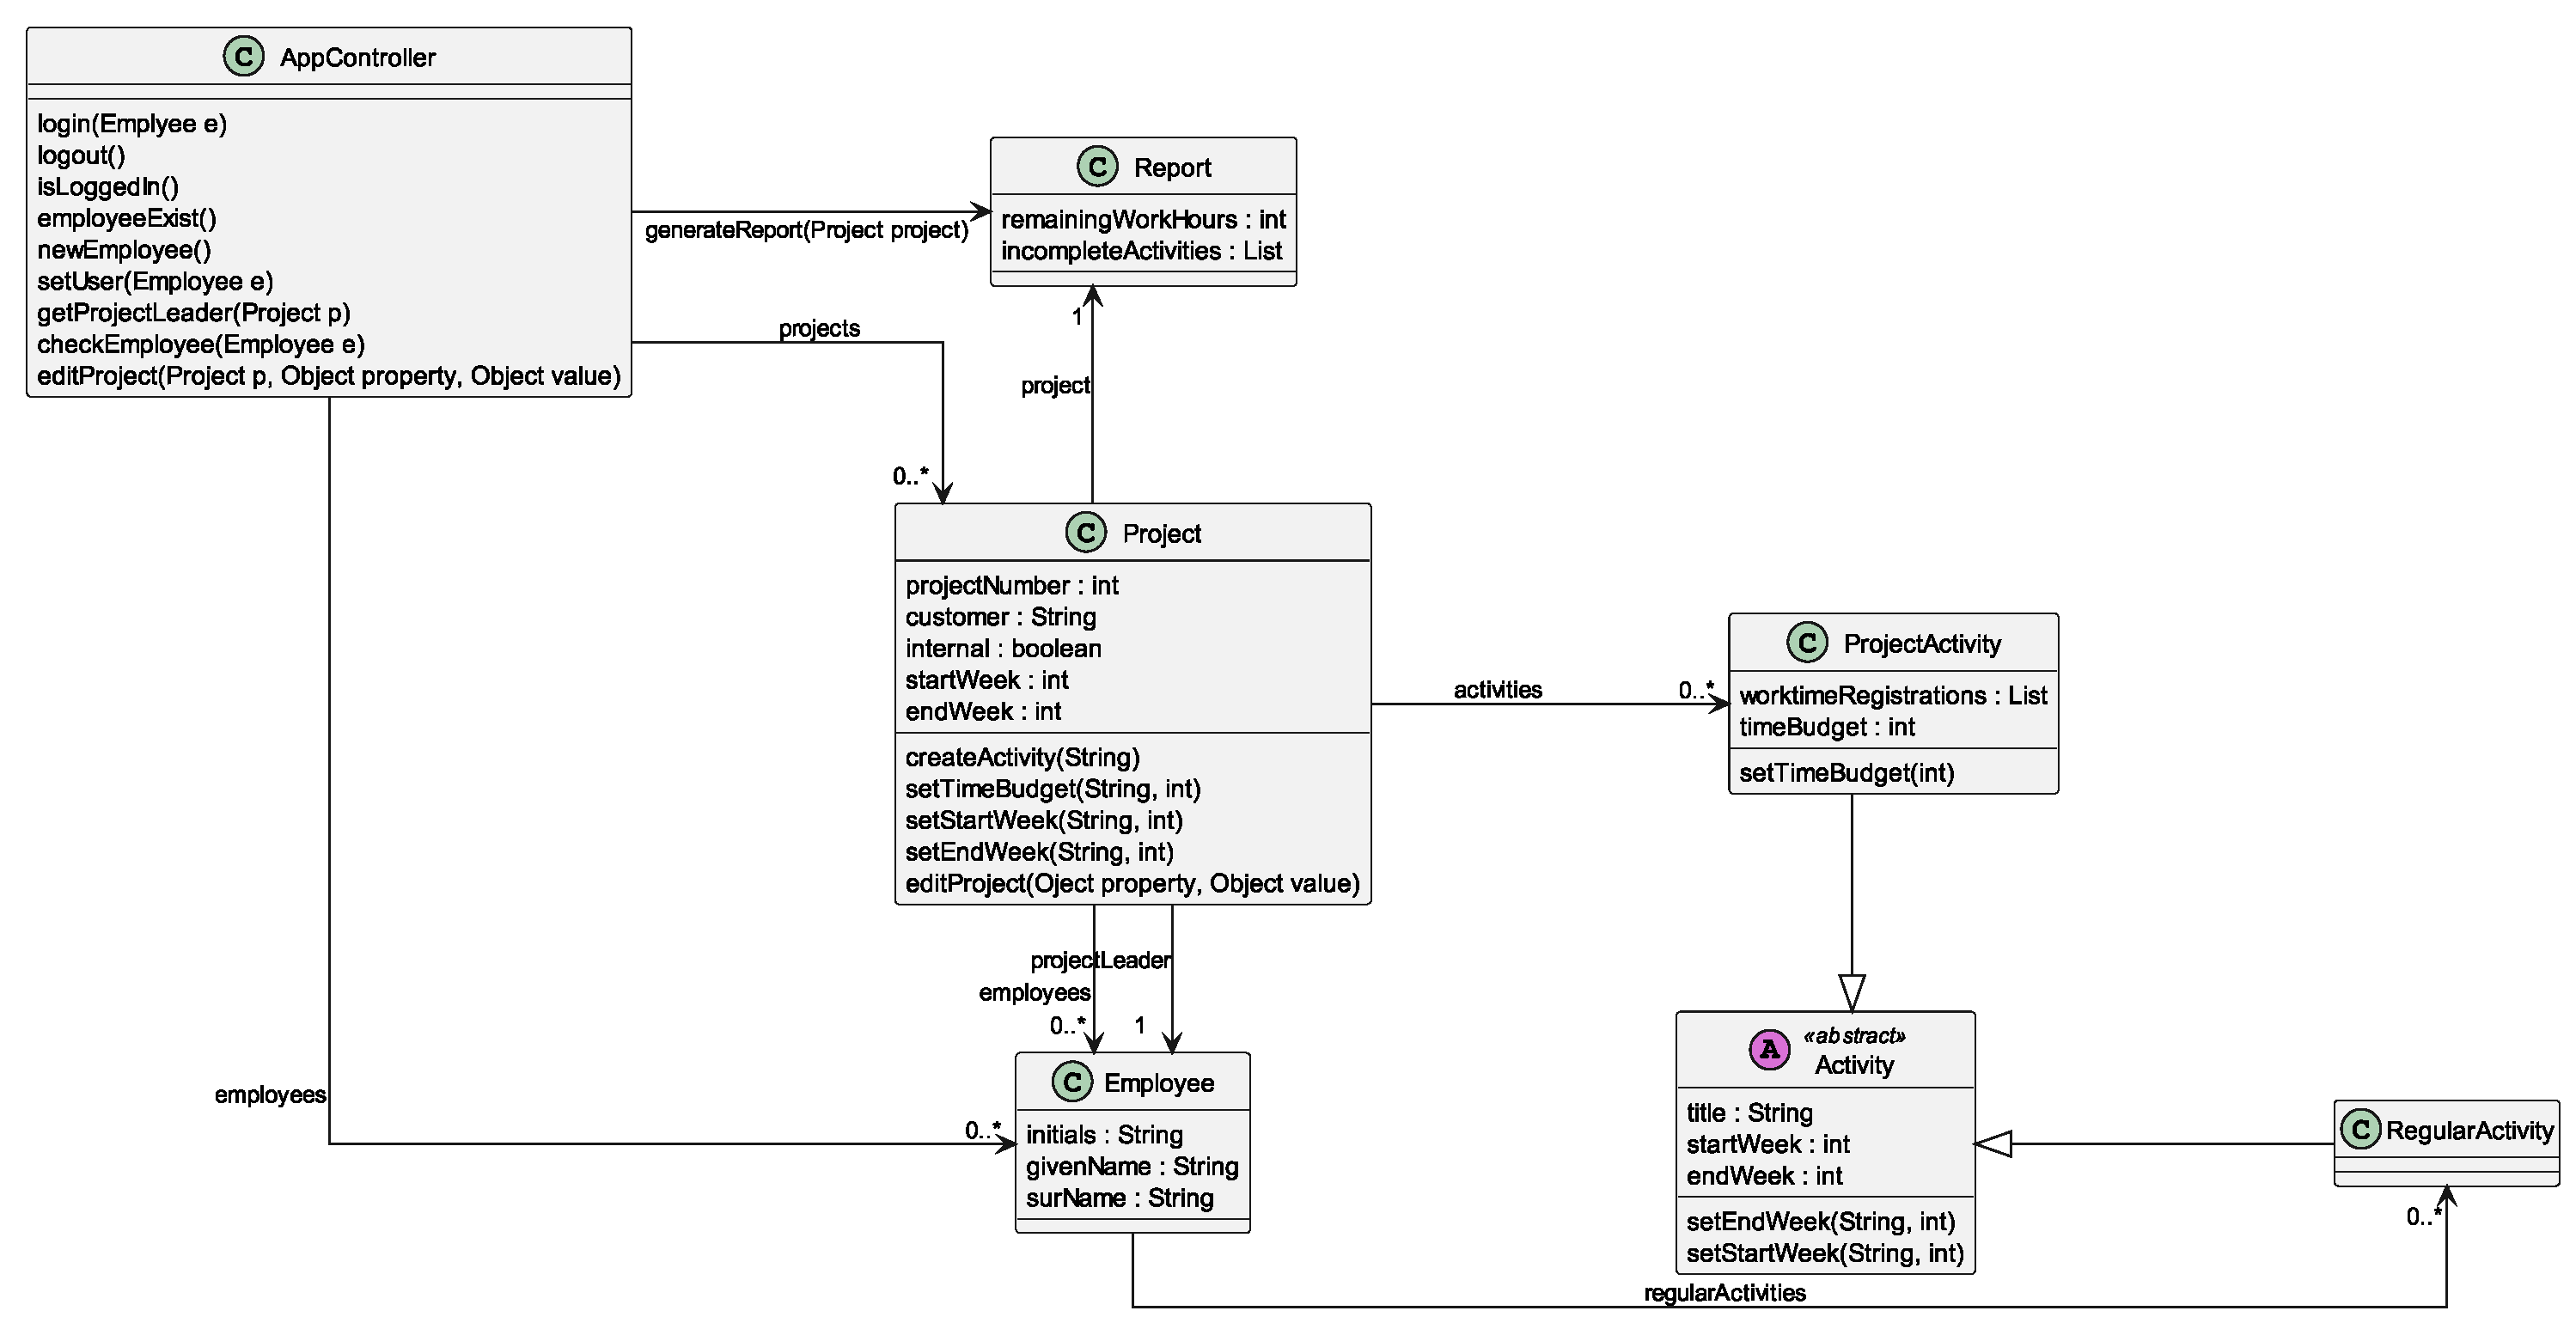
\includegraphics[width = 12cm, keepaspectratio]{RequirementsAndDesign/Diagrams/ClassDiagram.eps}
    \label{fig:class_report1}
\end{figure}
I takt med introduktion til \textit{Good Design}, \textit{Design patterns} og \textit{SOLID-principles} i undervisningen, har vi refaktoreret programmet for at forbedre designet. Det endelige design kan ses i appendix \ref{apdx:classDiagram_full}. Hovedsageligt er det \texttt{AppController}, der er trukket ud af \textit{domain}-laget, og opdelt til et \textit{facade}- og \textit{persistency}-lag. Med den indsigt vi har nu omkring program design, vil vi i projekter fremover være i bedre stand til at tænke god design ind fra starten.

Ser vi på funktionen \texttt{createRegularActivity()} i \texttt{Project} klassen, som vist i appendix \ref{apdx:seq_create_project_activity}. Her kan vi se metoden er ansvarlig for at verificere de argumenter der bliver givet, istedet for at gå ud fra, de allerede er verificeret. Det resulterer i, at en hel del kode eksekveres, inden de check nås, og \textit{Exceptions} da skal sendes hele vejen tilbage i forløbet. Men væsentligt er også, at metoden dermed har ansvar for mange forhold, hvilket kunne sepereres smartere. I forbindelse med introduktion af \textit{Design-By-Contract} begyndte vi blive opmærksomme på dette. Hvorfra mange af vores metoder er refaktoreret, til bedre at have styr på hvad de kan forvente og hvad der kan forventes af dem. 
Udover programlaget, er tilføjet et præsentationslag til håndtering af en brugergrænseflade. I denforbindelse oprettede vi \textit{ViewModels} for alle klasser i domæne-laget. For at opnå et bedre design, kan vi opdele disse domæne-klasser yderligere med en tilhørende \textit{Controller}-klasse, der kan have ansvar for disse argument valideringer, inden de bliver givet til selve modellen. Det vil desuden fuldende et \textit{MVC}-design mønster i domæne-laget, og gøre udbygning og vedligehold nemmere.